% Chapter Template

\chapter{Validació del sistema} % Main chapter title

Definits els components i detalls que componen el sistema de monitoratge i el sistema d'adaptabilitat, i un cop justificada des d'un punt de vista teòric la satisfacció dels nostres objectius, és el moment de presentar un exemple de cas d'ús i provar l'execució per validar el seu funcionament satisfactori i avaluar els resultats obtinguts.

\section{Presentació de cas d'ús}

Recordem la premissa genèrica del cas d'ús que volem que el nostre sistema satisfaci:

\begin{center}
\textit{Donada un \textbf{procés de monitoratge actiu} en un dels monitors del nostre sistema, i una proposta de \textbf{nova configuració} modelada, volem executar de forma automatitzada una \textbf{reconfiguració} d'aquell procés de monitoratge d'acord amb els \textbf{canvis computats respecte l'actual}.}
\end{center}

Per validar aquesta execució necessitem definir: un \textit{Base Model} que modeli l'estat actual del sistema (figura ~\ref{fig:Figura37}, una \textit{Feature Configuration} que modeli la darrera aplicada al sistema (figura ~\ref{fig:Figura37}, una \textit{Feature Configuration} que modeli la nova proposta de configuració del sistema (figura ~\ref{fig:Figura38}) i un \textit{Adaptability Model} que defineixi l'adaptació de models i la reconfiguració  de monitors (figura ~\ref{fig:Figura39}).\\

\begin{figure}
\centering
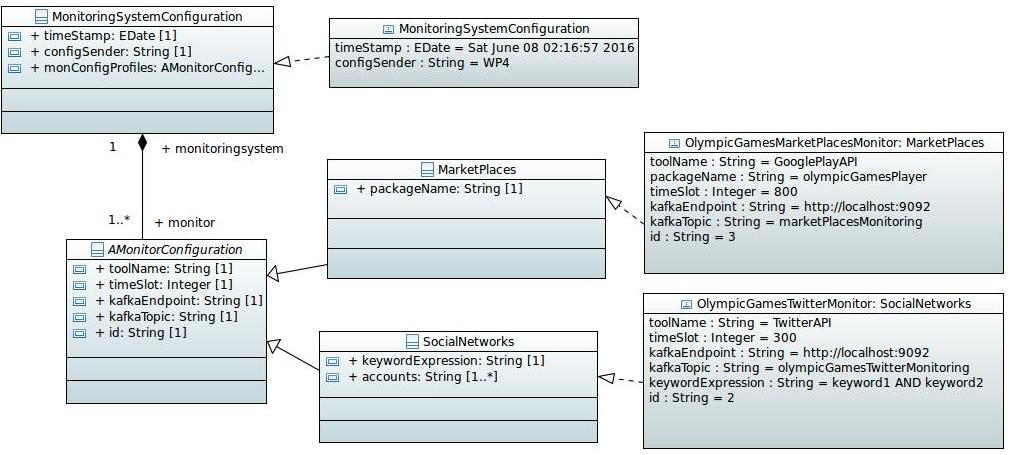
\includegraphics[width=14cm]{Figures/Figure16}
\decoRule
\caption{\textit{Base Model} utilitzat per validar la reconfiguració del sistema}
\label{fig:Figura36}
\end{figure} 

Com podem veure, el \textit{Base Model} defineix una configuració del sistema de monitoratge (ja vista anteriorment com a exemple en el \textit{Capítol 8. Modelatge UML de les configuracions de monitors}) amb dues instàncies de processos de monitoratge corrent: una sobre el monitor de Twitter, i l'altra sobre el monitor de Google Play, ambdues configurades amb els seus propis paràmetres de configuració. Pel nostre cas d'estudi, suposarem que aquest és el darrer \textit{Base Model} que defineix l'estat del sistema.\\

Si ens fixem en les dues \textit{Feature Configuration}, veiem que aquestes són pràcticament les mateixes, a excepció de l'atribut \textit{timeSlot} per les instàncies del monitor de Twitter que, en la nova proposta de configuració, pren un valor més elevat (de 30 segons passa a valer 50). S'ha triat aquest cas d'ús (la modificació del \textit{timeSlot}) per la validació del sistema per dos motius: primerament, per tractar-se d'un cas bàsic que permet observar amb detall la reconfiguració basant-nos en un únic punt de variabilitat, i segon perquè la modificació d'aquest \textit{timeSlot} serà fàcilment visualitzable en el procés d'execució dels monitors.\\ 

Finalment, l'\textit{Adaptability Model} descriu la \textit{feature} timeSlot com a \textit{feature} sobre la qual defineix una adaptació, així com els \textit{patterns} i rols a aplicar sobre els models, i finalment l'acció d'actualització del \textit{timeSlot} d'acord amb el valor definit.\\

\begin{figure}
\centering
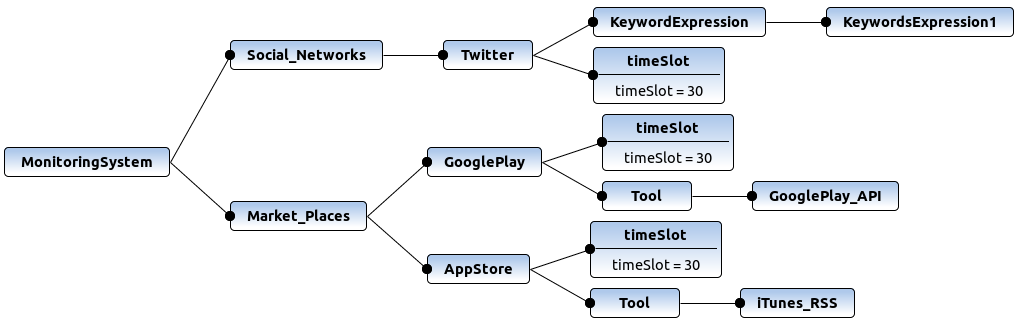
\includegraphics[width=14cm]{Figures/Figure36}
\decoRule
\caption{\textit{Feature Configuration} que descriu la darrera configuració del sistema aplicada}
\label{fig:Figura37}
\end{figure} 

\begin{figure}
\centering
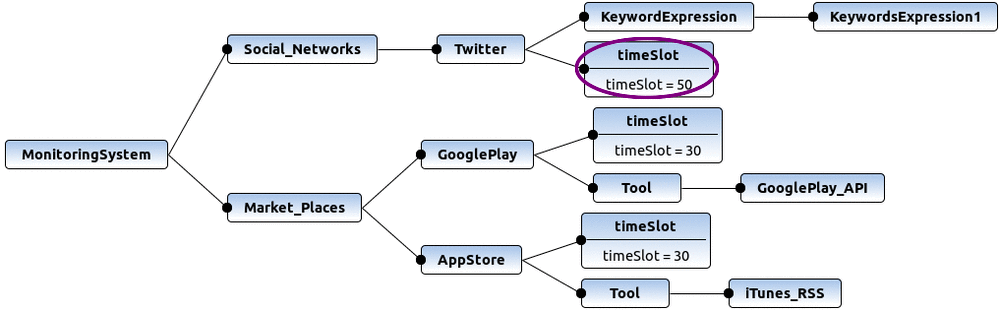
\includegraphics[width=14cm]{Figures/Figure37}
\decoRule
\caption{\textit{Feature Configuration} que descriu la configuració a aplicar per la reconfiguració}
\label{fig:Figura38}
\end{figure} 

\begin{figure}
\centering
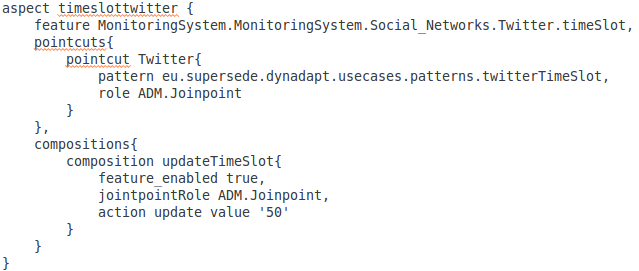
\includegraphics[width=14cm]{Figures/Figure38}
\decoRule
\caption{\textit{Adaptability Model} que descriu la reconfiguració a executar}
\label{fig:Figura39}
\end{figure} 

\section{Execució de la reconfiguració}

El disparador de l'execució serà la sol·licitud a través del \textit{dashboard} de la reconfiguració associada a la \textit{Feature Configuration} 

\begin{figure}
\centering
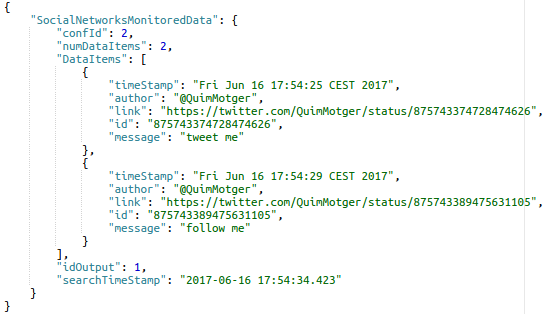
\includegraphics[width=11cm]{Figures/tfg1}
\decoRule
\caption{Primer enviament de dades del monitor de Twitter a Kafka}
\label{fig:tfg1}
\end{figure} 

\begin{figure}
\centering
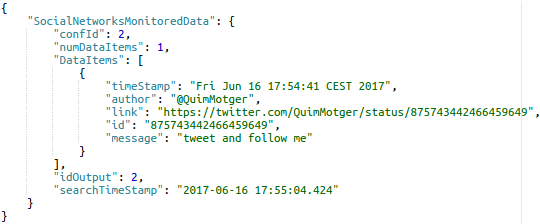
\includegraphics[width=11cm]{Figures/tfg2}
\decoRule
\caption{Segon enviament de dades del monitor de Twitter a Kafka (abans de la reconfiguració)}
\label{fig:tfg2}
\end{figure} 

\begin{figure}
\centering
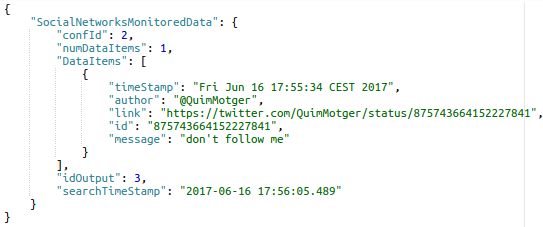
\includegraphics[width=11cm]{Figures/tfg3}
\decoRule
\caption{Tercer enviament de dades del monitor de Twitter a Kafka (després de la reconfiguració)}
\label{fig:tfg3}
\end{figure} 

\begin{figure}
\centering
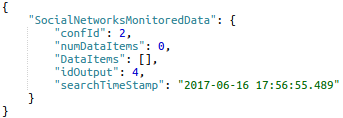
\includegraphics[width=8cm]{Figures/tfg4}
\decoRule
\caption{Quart enviament de dades del monitor de Twitter a Kafka (configuració estable)}
\label{fig:tfg4}
\end{figure} 